\let\negmedspace\undefined
\let\negthickspace\undefined
\documentclass[journal]{IEEEtran}
\usepackage[a5paper, margin=10mm, onecolumn]{geometry}
%\usepackage{lmodern} % Ensure lmodern is loaded for pdflatex
\usepackage{tfrupee} % Include tfrupee package

\setlength{\headheight}{1cm} % Set the height of the header box
\setlength{\headsep}{0mm}  % Set the distance between the header box and the top of the text

\usepackage{gvv-book}
\usepackage{gvv}
\usepackage{cite}
\usepackage{amsmath,amssymb,amsfonts,amsthm}
\usepackage{algorithmic}
\usepackage{graphicx}
\usepackage{textcomp}
\usepackage{xcolor}
\usepackage{txfonts}
\usepackage{listings}
\usepackage{enumitem}
\usepackage{mathtools}
\usepackage{gensymb}
\usepackage{comment}
\usepackage[breaklinks=true]{hyperref}
\usepackage{tkz-euclide} 
\usepackage{listings}
% \usepackage{gvv}                                        
\def\inputGnumericTable{}                                 
\usepackage[latin1]{inputenc}                                
\usepackage{color}                                            
\usepackage{array}                                            
\usepackage{longtable}                                       
\usepackage{calc}                                             
\usepackage{multirow}                                         
\usepackage{hhline}                                           
\usepackage{ifthen}                                           
\usepackage{lscape}
\begin{document}

\bibliographystyle{IEEEtran}
\vspace{3cm}

\title{9.2.18}
\author{EE24BTECH11021 - Eshan Ray}

% \maketitle
% \newpage
% \bigskip
{\let\newpage\relax\maketitle}

\renewcommand{\thefigure}{\theenumi}
\renewcommand{\thetable}{\theenumi}
\setlength{\intextsep}{10pt} % Space between text and floats




\textbf{Question: }\\
Find the area of the region bounded by the curve $x^2 = y$ and the lines $y = x + 2$ and
the $x-axis$.\\
\solution {
\begin{table}[h!]    
  \centering
  \begin{tabular}[12pt]{ |c| c|}
    \hline
        \textbf{Variable}  & \textbf{Description} \\
    \hline
        $\vec{B}$$\brak{-4,0}$ &  coordinates of first point  \\
    \hline 
        $\vec{C}$$\brak{10,0}$ & coordinates of second point \\
    \hline
        $\vec{A}$& Equidistant point of $\vec{B}$ and $\vec{C}$ on $X$ axis \\  
    \hline
         
\end{tabular}

  \caption{Input parameters}
  \label{tab1.1.9.2}
\end{table}
\\
The point of intersection of the line with the parabola is $x_i=h+k_i m$,\\
where,$k_i$ is a constant and is calculated as follows:-
$$k_i=\frac{1}{m^\top Vm}\brak{-m^\top \brak{Vh+u}\pm \sqrt{\sbrak{m^\top \brak{Vh+u}}^2-g\brak{h}\brak{m^\top Vm}}}$$\\
Substituting the input parameters in $k_i$,
\begin{multline}
     k_i =\frac{1}{\myvec{1&1}\myvec{1&0\\0&0}\myvec{1\\1}}\brak{-\myvec{1&1}\brak{\myvec{1&0\\0&0}\myvec{0\\2}+\myvec{0\\ \frac{-1}{2}}}\pm \\
     \sqrt{\sbrak{\myvec{1&1}\brak{\myvec{1&0\\0&0}\myvec{0\\2}+\myvec{0\\ \frac{-1}{2}}}}^2-g\brak{h}\brak{\myvec{1&1}\myvec{1&0\\0&0}\myvec{1\\1}}}} 
\end{multline}
We get,\\
$$k_i= -1, 2$$
Substituting $k_i$ in $x_i=h+k_i m$  we get,\\
\begin{align}
     x_1&=\myvec{0\\2}+\brak{-1}\myvec{1\\1}\\
    \implies x_1 &=\myvec{0\\2} + \myvec{-1\\-1}\\
    \implies x_1 &=\myvec{-1\\1}\\
    x_2 &=\myvec{0\\2}+\brak{2}\myvec{1\\1}\\
    \implies x_2&=\myvec{0\\2}+\myvec{2\\2}\\
    \implies x_2&=\myvec{2\\4}
\end{align}
The area bounded by the curve $y = x^2$ and line $y = x+2$ is given by
\begin{align}
    \int_{-1}^{2} x+2-x^2 \,dx &= \brak{\frac{x^2}{2}+2x-\frac{x^3}{3}}\limits_{-1}^{2} \ \\
    &= \brak{\frac{4}{2}+4-\frac{8}{3}}-\brak{\frac{1}{2}-2+\frac{1}{3}}\\
    &= \brak{\frac{10}{3}}-\brak{\frac{-7}{6}}\\
    &= \frac{9}{2} 
\end{align}

So, the required area is $4.50$ units.
   \begin{figure}[!ht]
    \centering
	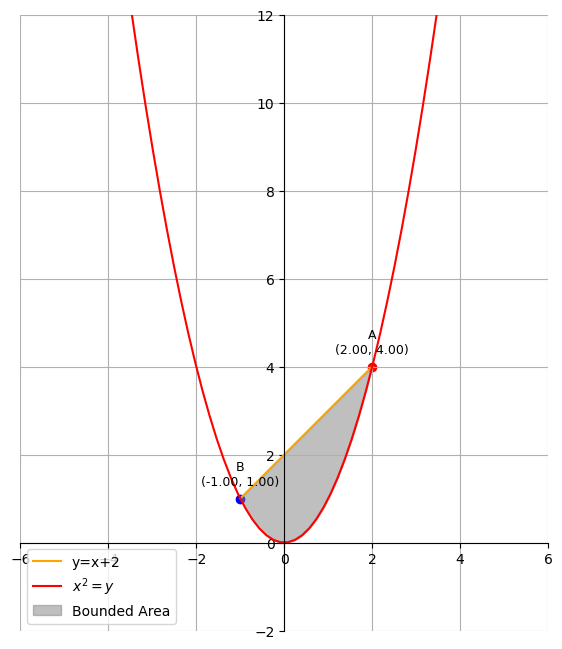
\includegraphics[width=1\textwidth]{plots/plot.png}
    \caption{Intersection of line and parabola}
    \label{fig:plot}
\end{figure}  

}
\end{document}
